\documentclass[a4paper,fleqn]{article}
%% Seitenaufbau
\usepackage[top=3cm, bottom=2.5cm, left=3.5cm, right=3.5cm]{geometry}

%% Schriftbild
\usepackage{lmodern}  % Latin Modern Zeichensatz
\usepackage[utf8]{inputenc}  % Unterstuetzung von Umlauten im Quelltext
\usepackage[T1]{fontenc}  % Korrekte Umlaute im Output
\renewcommand{\familydefault}{\sfdefault}  % Serifenlose Schrift
\usepackage{setspace}\onehalfspacing  % 1.5-facher Zeilenabstand
\renewcommand{\arraystretch}{1.5}  % 1.5-facher Zeilenabstand (Tabellen)
\setlength{\parindent}{0pt}  % Keine Einrueckung am Beginng von Absaetzen
\usepackage{fancyhdr}
\pagestyle{fancy}
\renewcommand{\headrulewidth}{0.5pt}
\renewcommand{\sectionmark}[1]{\markright{\thesection\ #1}}
\lhead{\rightmark}
\chead{}
\cfoot{\thepage}  % Richtige Schriftart fuer Seitenzahlen
\sloppy  % Weniger strikte Silbentrennung

%% Verlinkung von Inhaltsverzeichnis, Bildern und Formeln
\usepackage[pagebackref]{hyperref}  % Verlinkung von URLs und Referenzen
\usepackage{color}  % Definition von Linkfarben
\definecolor{DarkRed}{rgb}{0.5,0,0}
\hypersetup{
  colorlinks,
  citecolor=DarkRed,
  linkcolor=DarkRed,
  urlcolor=blue}

%% Mathematikumgebung
\usepackage{mathtools}
\usepackage{amssymb}  % Erweiterte Bibliothek mathematischer Symbole
\usepackage{euler}  % Serifenlose Schrift in Formelumgebungen
\renewcommand{\epsilon}{\varepsilon}  % Nutze "richtiges" Epsilon

%% Grafikumgebungen
\usepackage{graphicx}  % Erweiterte Grafikumgebung
\usepackage{float}  % Automatische Positionierung von Bildern
\usepackage{floatflt}  % Grafiken im Text einbetten
\usepackage{subcaption}  %  Bildunterschriften fuer subfigures

%% Listenumgebung
\usepackage{enumerate}
\usepackage{textcomp}  % Korrekte serifenlose Aufzählungszeichen

%% Farbige Umrahmungen
\usepackage{framed}
\definecolor{shadecolor}{rgb}{0.9,0.9,0.9}

%% Chemische Formeln
\usepackage{chemfig}

%% Inhalt der Titelseite
\title{Advanced radiation and remote sensing}
\author{Stefan A Buehler, Lukas Kluft, Christoph Sauter, Jakob Doerr, FIXME all that worked on
the script}
\date{\today}

%%%%%%%%%%%%%%%%%%%%%%%%%%%%%%%%%%%%%%%%%%%%%%%%%%%%%%%%%%%%%%%%%%%%%%
\begin{document}
\maketitle
\thispagestyle{empty}\pagestyle{empty}
\tableofcontents
\newpage\pagestyle{fancy}

% CHAPTER 1 - INTRODUCTION
\section{Introduction}

FIXME

% CHAPTER 2 ROTATIONAL SPECTRA
\section{Rotational spectra}

\subsection{Energy states and photons}
Absorption and emission of a photon can happen if the internal energy of a
molecule changes. The difference in two energy states $E$ and the frequency of
the photon $\nu$ are connected through the Planck constant $h$.
\begin{equation}
  E_f - E_i = \Delta E = h \nu
\end{equation}
The transition between different energy levels can be divided into three types,
corresponding to different states of the molecule.  Each transition type is
characteristic for a specific region of the electro-magnetic spectra.  One can
distinguish changes in a molecules rotation (microwave), vibration (infrared)
and electronic transitions (UV/visible).

Molecules consist of different atoms. There are diatomic molecules with two
atoms ($O_2$, $N_2$, $NO$, $HCl$, $CO$) and polyatomic molecules with
three or more atoms ($O_3$, $NO_2$, $CO_2$). We will mainly discuss
diatomic molecules, because they are easier to understand.

One can distinguish between three types of interaction between a photon and a
molecule: absorption, spontaneous emission and stimulated emission.  There are
three conditions to be fulfilled for a molecule to absorb a photon:
\begin{enumerate}
\item The frequency of the photon has to match one the molecule's energy
transitions.
\begin{equation}
  \Delta E = h \nu
\end{equation}

\item The net absorption has to be proportional to the difference of occupation
probabilities of states $i$ and $f$: $p_i - p_f$. Where $p_i$ is given by the
Boltzmann distribution (in local thermodynamic equilibrium).
\begin{equation}
  p_i = \frac{q_i e^{-E_i / (kT)}}
        {\sum_{j=1}^\infty q_j e^{-E_j / (kT)}}
\end{equation}
The denominator is often referred to as $Q(T)$. It has various names like total
internal partition sum, partition function, or Zustandssumme.

\item Absorption is proportional to the electric dipole matrix element $\mu_{if}$
between states $i$ and $f$.
\begin{equation}
  \mu_{if} = \mu \iiint \psi_f^*(x,y,z) \psi(x,y,z) \,dx\,dy\,dz
\end{equation}
Where $\mu$ is the magnitude of the dipole operator. $\mu_{if}$ is a constant
for each transition.
\end{enumerate}

Combining all conditions, one can define the absorption coefficient $\alpha$.
\begin{equation}
  \alpha(\nu) = n \sum_{f,i} S_{fi}(T) \delta(\nu_{fi} - \nu)
\end{equation}
With number density $n$, line strength $S_{fi}$, difference of state energies
$h\nu_{fi}$ and Dirac's delta function $\delta$ (physical not true, will be
replaced later by a so called "line shape" function.

The line strength is different for each transition and defined as follows.
\begin{equation}
    S_{fi} = \frac{8\pi^3\nu_{fi} \lvert\mu_{fi}\rvert^2 q_i}{3hcQ(T)}
      \left( e^{E_i/(kT)} - e^{E_f/(kT)} \right)
\end{equation}
Although this equations looks complicated, there is only one true independent
variable, the temperature $T$. All other variables are constants of the
transition, or fundamental constants.

Spectral line catalogues are collections of these transition parameters. There
is one line in the catalogue for each spectral line (thousands for each
molecule). The most well-known is the HITRAN catalogue.


\subsection{Rotational transitions}
\begin{figure}[htbp]
\begin{center}
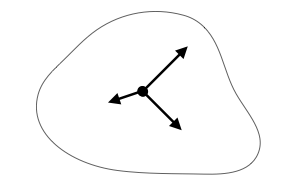
\includegraphics[width=0.4\textwidth]{figures/Fig_moments_inertia}
\caption{FIXME}
\label{default}
\end{center}
\end{figure}

Every free molecule has 3 \textbf{Moments of inertia} $I_A$, $I_B$, $I_C$ (\textit{Trägheitsmomente}), since there are 3 principal axes of rotation in the x-y-z-plane. We can use the Moments of inertia to classify the molecules and devide them into groups:


\begin{center}
\begin{tabular}{| c | c | c | c |}
  \hline
  Linear & Spherical top & Symmetric top & Asymmetric top \\
  \hline
  & & &  \\
\chemfig{H-[,0.8]Cl} &
\chemfig{C(-[:330]H)(-[:90,0.8]H)(-[:210]H)(-[:270,0.8]H)} &
\chemfig{C(-[:0,0.8]F)(-[:140]H)(-[:180,0.8]H)(-[:220]H)} &
\chemfig{H-[:30,0.8]O-[:-30,0.8]H} \\
 & & & \\
  %\hline
  $I_A \approx 0$,   $I_B = I_C$ &
  $I_A = I_B = I_C$ &
  $I_A \neq 0$,   $I_B = I_C \neq I_A$ & 
  $I_A \neq I_B \neq I_C$ \\
  \hline
\end{tabular}
\end{center}

From classical mechanics, we can define the Rotational energy
\begin{equation}
E_r = \frac{1}{2} I \omega^2 = \frac{J^2}{2I},
\end{equation}
where $\omega$ is the angular frequency (\textit{Kreisfrequenz}), $I$ the moment if inertia and $J = I\cdot\omega$ the angular momentum (\textit{Drehmoment}).\\

\begin{figure}[htbp]
\begin{center}
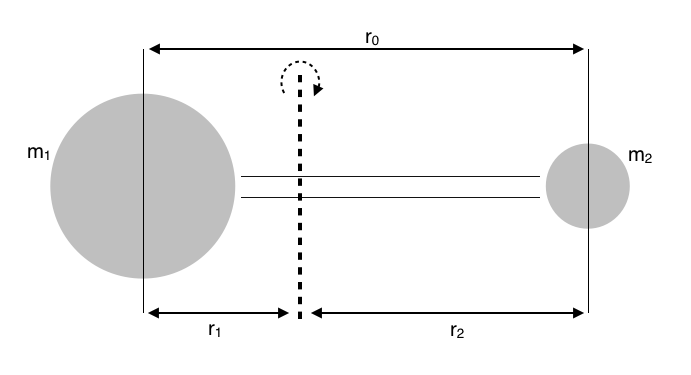
\includegraphics[width=1\textwidth]{figures/Reduced_mass}
\caption{FIXME}
\label{default}
\end{center}
\end{figure}

In case of a diatomic molecule, we can use the \textbf{reduced mass $\mu$} to express some properties of the molecule more easily. The relative motion of such a diatomic molecule is the same as that of a simple particle with the reduced mass $\mu$. It can be calculated by taking into account the two individual masses $m_1, m_2$ of the individual atoms.
\begin{equation}
\mu = \frac{m_1 m_2}{m_1+m_2} \qquad or \qquad \frac{1}{\mu} = \frac{1}{m_1} + \frac{1}{m_2}
\end{equation}
If we devide the distance between the mass centers of the atoms $r_0$ into their individual distances to the axis of rotation $r_1, r_2$, so that $r_0 = r_1 + r_2$, we can define the center of gravity:
\begin{equation*}
m_1 r_1 = m_2 r_2
\end{equation*}
The general formula for the moment of inertia 
\begin{equation*}
I = \sum_i m_i r_i^2 
\end{equation*}
can therefore be expressed as 
\begin{equation}
I = \mu r_0^2.
\end{equation}
Now we look at two extreme cases for the reduced mass:
\begin{enumerate}
\item The masses of both atoms are equal ($m_1 = m_2$) \\
  $\Rightarrow \mu = \frac{m_1^2}{2m_1} = \frac{1}{2}m_1 = \frac{1}{2}m_2$
\item One mass is much larger than the other ($m_1 >> m_2$) \\
  $\Rightarrow \mu = \frac{m_2}{\frac{m_1 + m_2}{m_1}} \approx m_2$ 
\end{enumerate}
In Quantum mechanics, you can express energy levels by using the Hamiltonian function (total energy)
\begin{equation}
\mathcal{H}=\frac{J^2}{2I},
\end{equation}
which leads to a discrete number of allowed energy solutions:
\begin{equation}
E_\mathcal{J} = \frac{\hbar^2}{2I} \mathcal{J}(\mathcal{J}+1), \qquad \text{with} \quad \mathcal{J} = 0, 1, 2, ...
\end{equation}
$\hbar$ = $h/2\pi$ is the Planck constant and $\mathcal{J}$ the rotational quantum number. \\
Energy(diferences) can be conveniently expressed in \textbf{wavenumbers} (Kaisers)
\begin{equation}
\tilde{\nu} = \frac{\Delta E}{hc} \qquad \left[\frac{1}{cm}\right]
\end{equation}
or in frequency (Hz)
\begin{equation}
\nu = \frac{\Delta E}{h} \qquad \left[Hz\right],
\end{equation}
so they translate directly to the observed spectrum.\\
The energy levels can be expressed in wavenumbers by
\begin{equation}
\epsilon_\mathcal{J} = \frac{E_\mathcal{J}}{hc} = \frac{h}{\delta \pi^2 I c} \mathcal{J}(\mathcal{J}+1).
\end{equation}
$\delta$ is Dirac's delta function and c the speed of light in vacuum. The fracture on the right side of the equation is referred to as the rotational constant B. It is inversely proportional to the moment of inertia $I$. From Quantum mechanics it turns out, that the only transitions that are allowed are those where $\Delta \mathcal{J} = \pm1$. Therefore we can only get energy levels $\epsilon_J$ that are 0, 2B, 6B, 12B, 20B, ..., all other transitions are forbidden, which results in equidistant spectral lines. \\

\begin{figure}[htbp]
\begin{center}
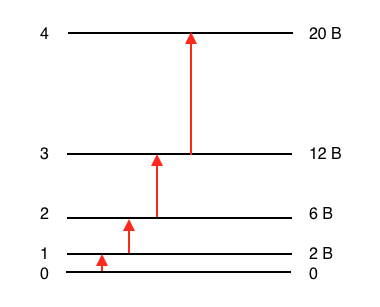
\includegraphics[width=0.5\textwidth]{figures/Energy_levels}
\caption{Values for $\mathcal{J}$ given on the left and the energy levels $\epsilon_{\mathcal{J}}$ in wavenumbers on the right.}
\label{default}
\end{center}
\end{figure}

This is an example of the selection rule. So the full spectrum of a diatomic molecule is given by
\begin{equation}
\tilde{\nu}_{\mathcal{J}\rightarrow \mathcal{J}+1} = 2B(\mathcal{J}+1), \qquad \mathcal{J} = 0, 1, 2, ...\,.
\end{equation}






% CHAPTER 3 - VIBRATIONAL SPECTRA
\section{Vibrational spectra}
Now we will turn to vibration, another mode of molecular internal energy. Just like rotational energy, vibrational energy is quantified, hence can lead to spectroscopic transitions (= absorption lines). \\
We start off by looking at a harmonic oscillator in regular mechanics. Assume there is a restoring force,
\begin{equation}
f = -k (r-r_{eq}) \qquad (\text{Hooke's law})
\end{equation}
at the point $r$ from the equilibrium point $r_{eq}$ with a constant $k$, then the associated energy is
\begin{equation}
E = \frac{1}{2}k (r-r_{eq})^2 .
\end{equation}

\begin{figure}[htbp]
\begin{center}
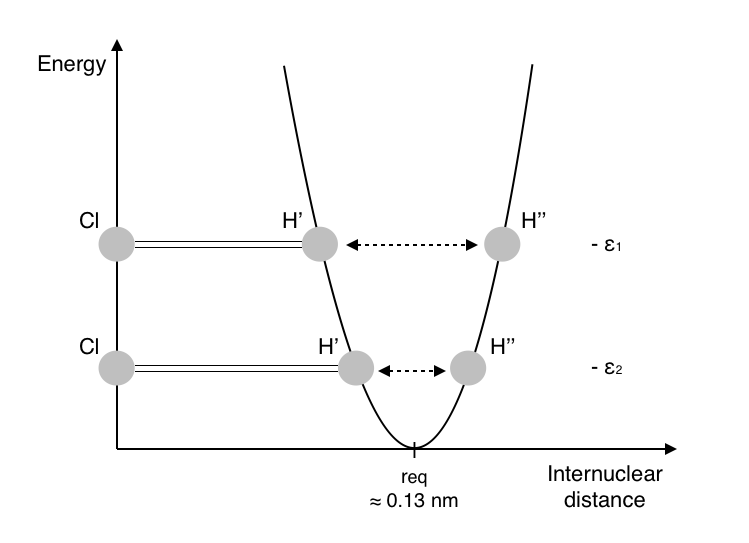
\includegraphics[width=1\textwidth]{figures/Vibration_parabol}
\caption{Energy curve for HCl molecules for extension or compression. After Banwell and McCash.}
\label{default}
\end{center}
\end{figure}

In Quantum Mechanics energy levels turn out to be 
\begin{equation}
E_\nu = (\nu+\frac{1}{2})\hbar\tilde{\omega} \qquad (\nu = 0, 1, 2, ...).
\end{equation}
Transformed into spectroscopic units of Kaiser we get
\begin{equation}
\epsilon_\nu = \frac{E_\nu}{hc} = (\nu + \frac{1}{2})\tilde{\nu}.
\end{equation}
So what is $\omega$? If $f$ is really proportional to $\Delta r$, then it is a constant:
\begin{equation}
\tilde{\omega} = \sqrt{\frac{k}{\mu}}
\end{equation}
FIXME: What are the names of $k$ and $\mu$?\par
The lowest vibrational level is at
\begin{equation}
E_0 = \frac{1}{2} \hbar \tilde{\omega}.
\end{equation}
Therefore a molecule can never have \textbf{zero} vibrational energy! This is different from rotation, where the lowest state had zero energy. \par

\begin{figure}[htbp]
\begin{center}
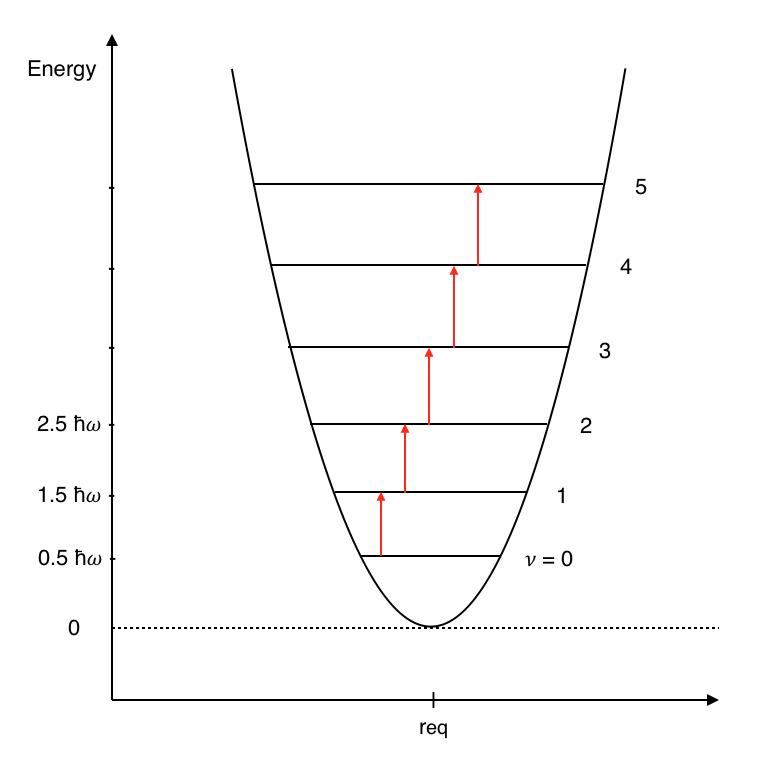
\includegraphics[width=0.8\textwidth]{figures/Vibration_parabol_2}
\caption{Allowed vibrational energy levels and transitions between them. After Banwell and McCash.}
\label{default}
\end{center}
\end{figure}

The frequency of the observed line corresponds to the energy difference $\tilde{\nu}$ between adjacent levels (which corresponds to the classical frequency at which the molecule would vibrate. If molecules rotate, the Energy separation is 1 - 10\,cm$^{-1}$ whereas if they vibrate, the Energy separation is 100 - 10\,000\,cm$^{-1}$. This is a large difference in characteristic energy. We can therefore assume that the two motions occur independently.
 (This is a case of the Born- Oppenheimer approximation, which strictly also includes vibration. We write
 \begin{gather}
E_{total} = E_{rot} + E_{vib} \qquad \left[J\right]  \\
\epsilon_{total} = \epsilon_{rot} + \epsilon_{vib} \qquad \left[cm^{-1}\right].
 \end{gather}
Combining the discrete energy levels results in
\begin{equation}
\epsilon_{\mathcal{J},\nu} = \epsilon_{\mathcal{J}} + \epsilon_{\nu} = B \mathcal{J} (\mathcal{J} + 1) + (\nu + \frac{1}{2})\tilde{\nu}.
\end{equation}
Note: There are higher order therms in both rotation (zentrifugal stretching) and vibration (non-constant restoring force) that I am ignoring here. \par
 
 \begin{figure}[htbp]
\begin{center}
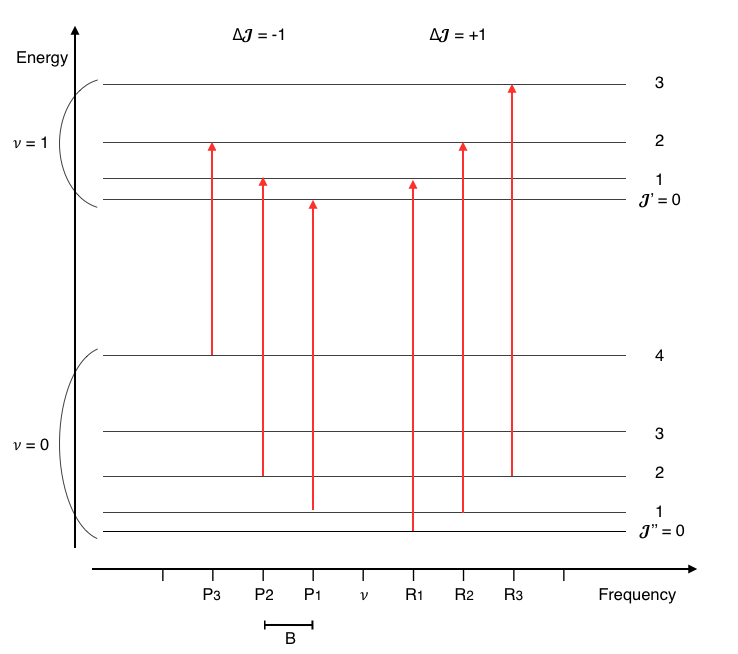
\includegraphics[width=1\textwidth]{figures/Transitions_vib_rot}
\caption{Transitons between vibrational - rotational energy levels. After Banwell and McCash.}
\label{default}
\end{center}
\end{figure}
 
 The selection rule states, that
 \begin{equation}
\Delta \nu = \pm 1 \text \quad {and} \quad \Delta \mathcal{J} = \pm 1.
\end{equation}
This means, we normally cannot observe the vibrational fundamental directly. Rotational levels will be filled to varying degrees in a population of molecules. This results in different line intensities. \\
The transition frequencies are divided into two branches:
\begin{gather*}
\Delta \mathcal{J} = +1 \quad (\text{R-Branch}) \\
\qquad \Delta \epsilon_{\mathcal{J},\nu} = \tilde{\nu} + 2 B ( \mathcal{J''} + 1), 
	\qquad \mathcal{J''} = 0, 1, 2  \\
\Delta \mathcal{J} = -1 \quad (\text{P-Branch}) \\
\qquad \Delta \epsilon_{\mathcal{J},\nu} = \tilde{\nu} - 2 B ( \mathcal{J'} + 1) , 
	\qquad \mathcal{J'} = 0, 1, 2  \\ 
\end{gather*}
 They can be combined into: 
 \begin{equation}
\Delta \epsilon_{\mathcal{J},\nu} = \tilde{\nu} + 2 B m , 
	\qquad m = \pm1, \pm2, \pm3, ...
\end{equation}
These are the frequencies of the observed lines. \\
So why are the branches called 'P' and 'R'? For more complicated molecules, $\Delta \mathcal{J} = 0 \text{ and } \pm 2$ may also be allowed. All possible branches are:


\begin{center}
\begin{tabular}{|c|c|c|c|c|c|} \hline
$\Delta\mathcal{J}$ = & -2 & -1 & 0 & +1 & +2 \\
\hline
Name & O & P & Q & R & S \\
\hline
\end{tabular}
\end{center}

H$_2$O and CO$_2$ have three fundamental vibrations. These are:

\begin{center}
\begin{tabular}{| c | c | c | }
  \hline
  Symmetric stretch & Symmetric bend & Antisymmetric stretch  \\
  \hline
  % H2O
\schemestart
\chemfig{@{a1}H-[:30,0.8]@{a2}O-[:-30,0.8]@{a3}H}
\arrow(@a1.south west--.south west){->}[210,0.6,line width=.4pt,blue]
\arrow(@a2.north--.north){->}[90,0.6,line width=.4pt,blue]
\arrow(@a3.south east--.north east){->}[-30,0.6,line width=.4pt,blue]
\schemestop &
\schemestart
\chemfig{@{a1}H-[:30,0.8]@{a2}O-[:-30,0.8]@{a3}H}
\arrow(@a1.north--.north){->}[90,0.6,line width=.4pt,blue]
\arrow(@a2.south--.south){->}[-90,0.6,line width=.4pt,blue]
\arrow(@a3.north--.north){->}[90,0.6,line width=.4pt,blue]
\schemestop &
\schemestart
\chemfig{@{a1}H-[:30,0.8]@{a2}O-[:-30,0.8]@{a3}H}
\arrow(@a1.south west--.south west){->}[210,0.6,line width=.4pt,blue]
\arrow(@a2.north east--.east){->}[0,0.6,line width=.4pt,blue]
\arrow(@a3.north east--.north west){->}[145,0.6,line width=.4pt,blue]
\schemestop  \\
  $\tilde{\nu}_1 = 3651.7 \text{\,cm}^{-1}$ &
  $\tilde{\nu}_2 = 1595.0 \text{\,cm}^{-1}$ &
  $\tilde{\nu}_3 = 3755.8 \text{\,cm}^{-1}$ \\
  \hline
  %CO2
\schemestart
\chemfig{@{a1}O-[,0.8]@{a2}C-[,0.8]@{a3}O}
\arrow(@a1.west--.west){->}[180,0.6,line width=.4pt,blue]
\arrow(@a3.east--.east){->}[0,0.6,line width=.4pt,blue]
\schemestop &
\schemestart
\chemfig{@{a1}O-[,0.8]@{a2}C-[,0.8]@{a3}O}
\arrow(@a1.north--.north){->}[90,0.6,line width=.4pt,blue]
\arrow(@a2.south--.south){->}[270,0.6,line width=.4pt,blue]
\arrow(@a3.north--.south){->}[90,0.6,line width=.4pt,blue]
\schemestop &
\schemestart
\chemfig{@{a1}O-[,0.8]@{a2}C-[,0.8]@{a3}O}
\arrow(@a1.north west--.north){->}[0,0.6,line width=.4pt,blue]
\arrow(@a2.south east--.south){->}[180,0.6,line width=.4pt,blue]
\arrow(@a3.east--.east){->}[0,0.6,line width=.4pt,blue]
\schemestop \\
  $\tilde{\nu}_1 = 1330.0 \text{\,cm}^{-1}$ &
  $\tilde{\nu}_2 = 667.3 \text{\,cm}^{-1}$ &
  $\tilde{\nu}_3 = 2349.3 \text{\,cm}^{-1}$ \\
\hline
  
\end{tabular}
\end{center}




% CHAPTER 4 - LINE SHAPE
\section{Line shape}

There are three mechanisms that lead to a broadening of absorption lines:
\begin{description}
\item[•] Natural line width
\item[•] Pressure broadening
\item[•] Doppler broadening 
\end{description}

\subsection{Natural line width}

So far we know that the difference between two energy states $E_{f}$ and $E_{i}$ equanls the frequency $\nu$ times the Planck constant $h$:
\begin{equation}
h \nu = E_f - E_i
\end{equation}

So absorption (and emission) would happen at exactly one frequency and the line shape would be a delta-function. There is a fundamental quantum mechanical principle that prevents this from being true. Heisenbergs's uncertainty principle sais that one cannot know position and momentum of a particle simultaneously: 

\begin{equation}
\Delta x \Delta p \approx \hbar
\end{equation}

where $\hbar$ is the reduced Planck constant. Another manifestation of this principle is:

\begin{equation}
\Delta E \Delta t \approx \hbar = 10^{-34}~J/s
\end{equation}

Thus, the shorter the lifetime of a state, the more uncertain is its energy. 
The groundstate has an infinite lifetime, so its energy is exactly known:

\begin{equation}
\Delta t = \infty \rightarrow \Delta E = 0
\end{equation}

The first excited electronic state has a finite lifetime:

\begin{equation}
\Delta t = 10^{-8}~s \rightarrow \Delta E = \frac{\hbar}{\Delta t} = \frac{10^{-34}}{10^{-8}} = 10^{-26}~J
\end{equation}

and the frequency is

\begin{equation}
\Delta \nu = \frac{\Delta E}{h} = \frac{10^{-26}~J}{10^{-34}~Js} = 10^{8}~Hz
\end{equation}

This seems a large number at first sight, but electronic transitions typically have frequencies of $10^{14}$-$10^{16}$~Hz (visible spectral range). 
Therefore natural line width can be considered as small. However, the actual shape of the line is important.  \\

The finite lifetime of the upper state means that it decays with time:
 
\begin{equation}
\frac{dn(t)}{dt} = -A n(t)
\end{equation}

where $n$ is the number of molecules in the excited state and A is the Einstein A coefficient for spontaneous emission. The solution of this equation is:
\begin{equation}
n(t) = n(0) e^{-At} = n(0) e^{\frac{t}{\tau}}
\end{equation}

where $\tau$ is the lifetime. $\frac{dn(t)}{dt}$ is the rate at which the excited state decays, but at the same time it is also the rate of spontaneously emitted photons (whenever a state decays, a photon is emitted). Thus, for the radiation flux L we can write: 

\begin{equation}
L(t) = L(0) e^{-At} 
\end{equation}

So L also decays exponentially in time. If a signal amplitude is not constant in time, it cannot be monochromatic. The frequency spectrum is given by the Fourier transform: 

\begin{equation}
F_{L}(\nu) = \frac{1}{\pi} \frac{A/4\pi}{(\nu - \nu_{0})^{2} + (A/4\pi)^{2}} = \frac{1}{\pi} \frac{\gamma_{N}}{(\nu - \nu_{0})^{2} + \gamma_{N}^{2}} 
\end{equation}

$F_{L}$ is called a Lorentz-Function (also Cauchy distribution or Breit Wigner distribution). $\gamma_{N}$ is the natural line width parameter. 

\subsection{Doppler Broadening}

Doppler Broadening is conceptually simpler than natural broadening. It is due to the thermal motion of the molecules, which Doppler-shifts the frequency (at any point in time one part of the molecules is moving towards me and one part is moving away). The Maxwell-distribution for velocity (valid for LTE) is:

\begin{equation}
p(n) = \sqrt{\frac{m}{2\pi kT}} \,\, exp(\frac{-mn^{2}}{2kT})  
\end{equation}

where n is the velocity and m is the mass of the molecule. 
Non-relativistic Doppler-shift is given by:

\begin{equation}
\nu - \nu_{0} = \frac{\nu_{0}u}{c}
\end{equation}

The faster the molecule, the larger the Doppler-shift. Combining this with the Maxwell velocity distribution gives

\begin{equation}
F_{D}(\nu) = \frac{1}{\gamma_{D}\sqrt{\pi} \,\, exp(-(\frac{\nu - \nu_{0}}{\gamma_{D}})^{2})}
\end{equation}

Note that $F_{D}$ is a Gaussian. $\gamma_{D} = \frac{\nu}{c} \sqrt{\frac{2kT}{m}}$ is called "Doppler Width". 

\subsection{Pressure Broadening}

Collisions between molecules also limit the lifetime of energy states ("collisional broadening"). If one assumes that collisions themselves take no time, that there is no interaction between collisions and that collisions completely "reset" the state, then the resulting shape is again Lorentzian:

\begin{equation}
F_{D}(\nu) = \frac{1}{\pi} \frac{\gamma_{C}}{(\nu - \nu_{0})^{2} + \gamma_{C}^{2}} 
\end{equation}

The rate of collision is proportional to pressure. \\

Empirically $\gamma_{C}$ is calculated as follows:

\begin{equation}
\gamma_{C} = p \cdot AGAM (\frac{T_{ref}}{T})^{NAIR}
\end{equation}

where AGAM and NAIR are in the spectral line catalogue. (In reality there are some more parameters.) \\

So which of the broadening mechanisms do we use in reality? We neglect natural broadening, but have to use thermal and collisional broadening ($\gamma_{D}$ and $\gamma_{C}$). The shape then is a convolution of Lorentz and Gauss shape, called "Voigt-Function". There is no analytical form of this function, only numerical approximations. \\

In the exercise you will find out which effect of broadening dominates when. 

% CHAPTER 5 - THERMAL RADIATION
\section{Thermal radiation}

FIXME: Mostly covered by script from Bachelor lecture, but at least
state the Planck law here.\vspace{1cm}


We now want to look at the balance between Radiation and Temperature. If an object receives more radiation, its temperature rises. And a higher temperature results in a higher emission of radiation. We first look at a black body that absorbs all incoming radiation without any reflection. This is the case e.g. in a hollow space. If the Temperature is kept constant, there will be a radiative equilibrium between the walls and the radiation on the inside of the hollow space. This radiative equilibrium is \textit{only} dependent on the temperature, every other dependancy would be contradicting the laws of Thermodynamics.

The relationship between temperature and radiation is described in what now is known as \textit{Planck's law}:
\begin{equation}
I_{\nu} = B_{\nu}(T) = \frac{2h\nu^3}{c^2(e^{\frac{h\nu}{kT}}-1)}, 
               \hspace{3cm} B_{\nu}(T) = \frac{2hc^2}{\lambda^5(e^{\frac{hc}{\lambda kT}}-1)}
\end{equation}
$I_\nu$ is the spectral radiance [W\,m$^{-2}$\,sr$^{-1}$\,Hz$^{-1}$], B the Planck function, T the temperature, h the  Plack constant, $\nu$ the frequency, c the speed of light, k the Boltzmann constant and $\lambda$ the wave length.\\
There are different approximations for the equation. The Rayleigh-Jeans Approximation describes shows a similar behaviour for the spectral radiance for low frequencies:
\begin{equation}
I_{\nu} = B_{\nu, RJ}(T) = \frac{2kT}{c^2}\nu^2
\end{equation}
Wien's displacement law states that the black body radiation curve for different temperatures peaks at a frequency proportional to the temperature.
\begin{equation}
\nu_{max} \propto T
\end{equation}
When radiation meets a surface, it is either absorbed or reflected. The absorption coefficient $\alpha$ therefore has values between 0 and 1. A body that emits thermal radiation has an emissivity coefficient $\epsilon$ between 0 and 1. An emissivity coefficient $\epsilon$ = 0 means no radiation is emitted, a body with $\epsilon$ = 1 emits the same amount of radiation a blackbody of same temperature would:
\begin{equation}
I_\nu = \epsilon(\nu)B_\nu(T)
\end{equation}
Absorption and Emissivity have to balanced, otherwise this would be contradicting to the second law of Thermodynamics. \textit{Kirchhoff's law of thermal radiation} states that for all frequencies and angles 
\begin{equation}
\epsilon(\vartheta,\varphi,\nu) = \alpha(\vartheta,\varphi,\nu).
\end{equation}

FIXME: Should 'Exkurs' (p25-36 script) also be covered? \vspace{1cm}

We now apply these rules to our climate system. The earth itself emits radiation at the temperature of its surface. Due to the natural greenhouse effect, the temperature at earth's surface is increased by 34\,K.
 \begin{figure}[htbp]
\begin{center}
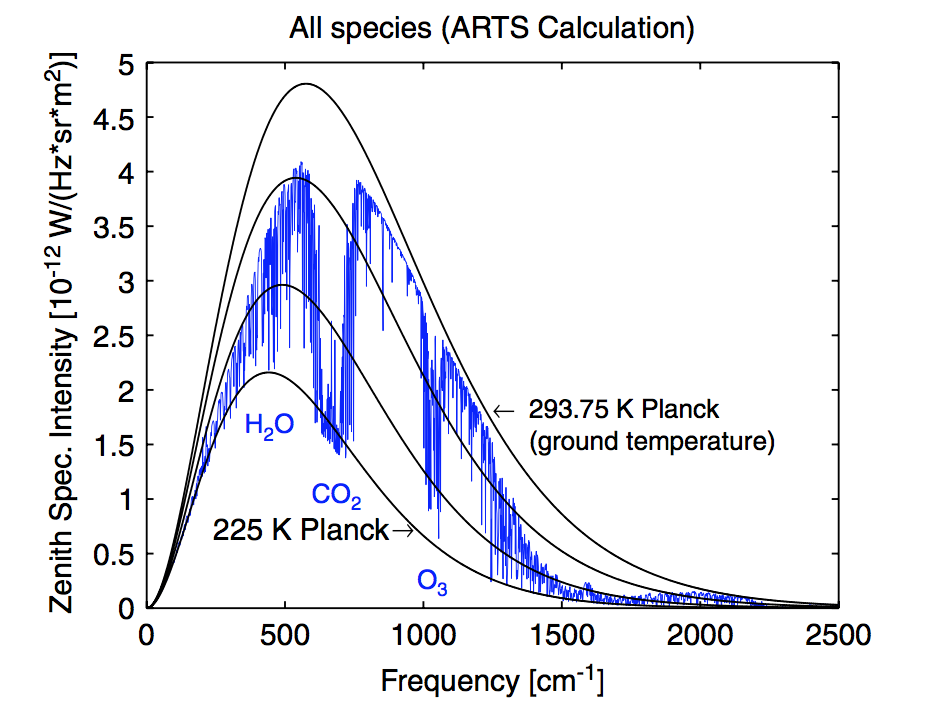
\includegraphics[width=1\textwidth]{figures/Buehler_et_al_OLR_spectra}
\caption{Clear-sky OLR spectra of the earth as seen from space. The area between the top curve and the blue curve is caused by the natural greenhouse effect. From Buehler et al., 2006.}
\label{default}
\end{center}
\end{figure}
Comparing the radiational intensities to the Planck curves shows at which temperature the radiation was emitted. 
\begin{equation}
T_b = B^{-1}_{\nu}(T)
\end{equation}
$T_b$ is called the brightnesstemperature. Using the brightnesstemperature in remote sensing is very common since it is an intuitive unit for the intensity. E.g. one would interpret $T_b = 300$\,K as a high value since there are not much higher temperatures in the atmosphere. $T_b = 200$\,K on the other hand, would not be very much.
 


% CHAPTER 6 - RADIATIVE TRANSFER EQUATION
\section{Radiative transfer equation}
The radiative transfer equation (RTE) describes the change of radiation along a path,
for example from the ground to a sensor above the surface. The RTE is expressed in 
terms of the monochromatic Intensity $I$. It can be written as
\begin{equation}
	\frac{dI}{ds} = - (\alpha + \sigma)I + \alpha B(T) + \sigma \int_\Omega PI 
	\frac{d\Omega}{4\pi}
\end{equation}
where $ds$ is a path element. The first term on the right hand side is 
the radiation loss due to extinction by absorption (absorption coefficient $\alpha$) 
and scattering (scattering coefficient $\sigma$). The second term is a source term
due to thermal emission $B(T)$. The third term is a source term due radiation that
is scattered into the path. It is calculated using the phase matrix $P$ of the 
scattering particles. The calculation involves an integration of the intensity over the 
whole solid angle $\Omega$. Note that normally, every variable depends on the frequency
and the viewing direction. \\
We see that if we include scattering in the RTE, it is very difficult to solve, because 
in order to compute the intensity in one direction, we need to know the intensity in 
every other direction.\\
One of the most used simplifications of the RTE is to neglect scattering. If we look at
thermal radiation, this is mostly true for a clear sky atmosphere. If we neglect 
scattering, the last term as well as the $\sigma$ in the first term vanish and the 
(clear sky) RTE looks like this:
\begin{equation}
	\frac{dI}{ds} = -\alpha I + \alpha B(T) = \alpha ( B(T) - I )
\end{equation}
This equation is also known as Schwarzschild's equation because if was formulated by 
K. Schwarzschild in 1906.\\
Using this equations, let's look at what happens in a homogeneous medium ($\alpha$ and $T$
constant). If the radiation passes through the medium long enough ($s \rightarrow \infty$)
the difference between $B$ and $I$ has to get smaller and smaller. This means that eventually,
$I$ will converge to $B$. This makes sense because if we look through a thick enough medium, 
we hardly see which radiation came into the medium, we only see the emission of the medium.\\
Schwarzschild's equation can be integrated along a path through a layer
(a complete derivation can be found in Petty, Eq. 8.5 - 8.13):
\begin{equation}
	I(s) = I(0) e^{-\tau (0,s)} + \int_{0}^{s} \alpha (s') B(s') 
	e^{-\tau (0,s')} ds' 
\end{equation}
where $\tau(0,s)$ is the opacity between the points. It is defined as:
\begin{equation}
	\tau (0,s) = \int_{0}^{s} \alpha(s') ds'.
\end{equation}
We see that the layer emits radiation, while the incoming radiation $I(0)$ is 
attenuated exponentially. \\
In radiative transfer models such as ARTS, the atmosphere is usually divided 
into homogeneous layers and the RTE is calculated through these layers. So to understand
the calculations in the model, it is useful to look at the solution of Schwarzschild's
equation in a homogeneous layer. The only difference is the opacity, which in a homogeneous
layer, we can write as
\begin{equation}
	\tau(0,s) = \int_{0}^{s} \alpha(s') ds' = \alpha s.
\end{equation}
To get the solution, we just plugin a homogeneous layer from 0 to $s$ into the integral 
form of the equation:
\begin{equation}
	I(s) = I(0) e^{-\alpha s} + \alpha B(T)\int_{0}^{s} e^{-\alpha (s-s')} ds' 
\end{equation}
which, after some algebra, gives this:
\begin{equation}
	I(s) = I(0) e^{-\alpha s} + B(T) \left( 1-e^{-\alpha s} \right).
\end{equation}
With the definition of the transmission $t = e^{-\alpha s}$, we can rewrite the solution as
\begin{equation}
	I(s) = t I(0)  + \left( 1-t \right) B(T).
\end{equation}
Let's look at a few extreme cases of the solution.\\
\underline{Optically thin:}\\
What happens if the opacity of the layer is very high, so $ t\rightarrow0$ ? 
Then we just see the Planck emission of the layer. the incoming radiation does not reach us.\\
\underline{Optically thin:}\\
What happens if the opacity of the layer is 0, to $ t \rightarrow \infty$ ? Then we just see
the incoming radiation $I(0)$. the layer doesn't do anything.\\
An interesting special case is when the opacity is small, but not zero. For small opacities, 
we can use a linear approximation of the transmission, which comes from the Taylor expansion
of the exponential function:
\begin{equation}
	t = e^{-\tau} \approx 1 - \tau.
\end{equation}
If we plug this into the solution of a homogeneous layer, we get
\begin{equation}
	I(s) = t I(0)  + \left( 1-t \right) B(T) \approx I(0) + \tau \left( B - I(0)\right)
\end{equation}
which has exactly the same form as Schwarzschild's equation itself.
%FIXME: Mostly covered by script from Bachelor lecture, but at least
%state the RTE here.

% CHAPTER 7 - JACOBIANS
\section{Jacobians}
 
\end{document}
